\documentclass{article}

% Packages required to support encoding
\usepackage{ucs}
\usepackage[utf8x]{inputenc}
\usepackage{graphicx} 
% Packages required by code

% Packages always used
\usepackage{listings}
\usepackage{hyperref}
\usepackage{xspace}
\usepackage[usenames,dvipsnames]{color}
\hypersetup{colorlinks=true,urlcolor=blue}


\usepackage[framed,numbered,autolinebreaks,useliterate] {mcode}


\usepackage{geometry}
\geometry{letterpaper,textwidth=350pt,textheight=680pt,tmargin=60pt,
            left=72pt,footskip=24pt,headsep=18pt,headheight=14pt}
\usepackage{amsmath}
\usepackage{amssymb}
\usepackage{textcase}
\usepackage{soul}

\newcommand{\mat}[1]{\boldsymbol{#1}}\renewcommand{\vec}[1]{\boldsymbol{\mathrm{#1}}}
\newcommand{\vecalt}[1]{\boldsymbol{#1}}

\newcommand{\conj}[1]{\overline{#1}}

\newcommand{\normof}[1]{\|#1\|}
\newcommand{\onormof}[2]{\|#1\|_{#2}}

\newcommand{\itr}[2]{#1^{(#2)}}
\newcommand{\itn}[1]{^{(#1)}}

\newcommand{\eps}{\varepsilon}
\newcommand{\kron}{\otimes}

\DeclareMathOperator{\diag}{diag}
\DeclareMathOperator{\trace}{trace}
\DeclareMathOperator{\tvec}{vec}

\newcommand{\prob}{\mathbb{P}}
\newcommand{\probof}[1]{\prob\left\{ #1 \right\}}

\newcommand{\pmat}[1]{\begin{pmatrix} #1 \end{pmatrix}}
\newcommand{\bmat}[1]{\begin{bmatrix} #1 \end{bmatrix}}
\newcommand{\spmat}[1]{\left(\begin{smallmatrix} #1 \end{smallmatrix}\right)}
\newcommand{\sbmat}[1]{\left[\begin{smallmatrix} #1 \end{smallmatrix}\right]}

\newcommand{\RR}{\mathbb{R}}
\newcommand{\CC}{\mathbb{C}}

\providecommand{\eye}{\mat{I}}
\providecommand{\mA}{\ensuremath{\mat{A}}}
\providecommand{\mB}{\ensuremath{\mat{B}}}
\providecommand{\mC}{\ensuremath{\mat{C}}}
\providecommand{\mD}{\ensuremath{\mat{D}}}
\providecommand{\mE}{\ensuremath{\mat{E}}}
\providecommand{\mF}{\ensuremath{\mat{F}}}
\providecommand{\mG}{\ensuremath{\mat{G}}}
\providecommand{\mH}{\ensuremath{\mat{H}}}
\providecommand{\mI}{\ensuremath{\mat{I}}}
\providecommand{\mJ}{\ensuremath{\mat{J}}}
\providecommand{\mK}{\ensuremath{\mat{K}}}
\providecommand{\mL}{\ensuremath{\mat{L}}}
\providecommand{\mM}{\ensuremath{\mat{M}}}
\providecommand{\mN}{\ensuremath{\mat{N}}}
\providecommand{\mO}{\ensuremath{\mat{O}}}
\providecommand{\mP}{\ensuremath{\mat{P}}}
\providecommand{\mQ}{\ensuremath{\mat{Q}}}
\providecommand{\mR}{\ensuremath{\mat{R}}}
\providecommand{\mS}{\ensuremath{\mat{S}}}
\providecommand{\mT}{\ensuremath{\mat{T}}}
\providecommand{\mU}{\ensuremath{\mat{U}}}
\providecommand{\mV}{\ensuremath{\mat{V}}}
\providecommand{\mW}{\ensuremath{\mat{W}}}
\providecommand{\mX}{\ensuremath{\mat{X}}}
\providecommand{\mY}{\ensuremath{\mat{Y}}}
\providecommand{\mZ}{\ensuremath{\mat{Z}}}
\providecommand{\mLambda}{\ensuremath{\mat{\Lambda}}}
\providecommand{\mPbar}{\bar{\mP}}

\providecommand{\ones}{\vec{e}}
\providecommand{\va}{\ensuremath{\vec{a}}}
\providecommand{\vb}{\ensuremath{\vec{b}}}
\providecommand{\vc}{\ensuremath{\vec{c}}}
\providecommand{\vd}{\ensuremath{\vec{d}}}
\providecommand{\ve}{\ensuremath{\vec{e}}}
\providecommand{\vf}{\ensuremath{\vec{f}}}
\providecommand{\vg}{\ensuremath{\vec{g}}}
\providecommand{\vh}{\ensuremath{\vec{h}}}
\providecommand{\vi}{\ensuremath{\vec{i}}}
\providecommand{\vj}{\ensuremath{\vec{j}}}
\providecommand{\vk}{\ensuremath{\vec{k}}}
\providecommand{\vl}{\ensuremath{\vec{l}}}
\providecommand{\vm}{\ensuremath{\vec{l}}}
\providecommand{\vn}{\ensuremath{\vec{n}}}
\providecommand{\vo}{\ensuremath{\vec{o}}}
\providecommand{\vp}{\ensuremath{\vec{p}}}
\providecommand{\vq}{\ensuremath{\vec{q}}}
\providecommand{\vr}{\ensuremath{\vec{r}}}
\providecommand{\vs}{\ensuremath{\vec{s}}}
\providecommand{\vt}{\ensuremath{\vec{t}}}
\providecommand{\vu}{\ensuremath{\vec{u}}}
\providecommand{\vv}{\ensuremath{\vec{v}}}
\providecommand{\vw}{\ensuremath{\vec{w}}}
\providecommand{\vx}{\ensuremath{\vec{x}}}
\providecommand{\vy}{\ensuremath{\vec{y}}}
\providecommand{\vz}{\ensuremath{\vec{z}}}
\providecommand{\vpi}{\ensuremath{\vecalt{\pi}}}

\sodef\allcapsspacing{\upshape}{0.15em}{0.65em}{0.6em}%

\makeatletter
\def\maketitle{%
\par
\hrule height 0.75pt\vspace{1ex}
\par\noindent
\begin{minipage}{0.5\textwidth}
\scshape
purdue university $\cdot$ CS 580 \\
Introduction to the Analysis of Algorithms
\end{minipage}
\begin{minipage}{0.5\textwidth}
\raggedleft
\MakeTextUppercase{\allcapsspacing{\@title}}\\[0.2ex]
\textit{\@author}\\[0.2ex]
\textit{\@date}
\end{minipage}
\par\vspace{1ex}
\hrule height 1pt
\vspace{2ex}
\par
}
\makeatother

\author{Jun Cheng}
\title{Lecture Notes}
% auto generate a title
\AtBeginDocument{\maketitle}


\title{Homework}



\begin{document} 



\hypertarget{problem_0_homework_checklist_2}{}
\subsection*{{Problem 0: Homework checklist}}
\label{problem_0_homework_checklist_2}

\checkmark	I didn't talk with any one about this homework. \newline
\checkmark 	Source-code are included at the end of this document. 

\hypertarget{}{}
\subsection*{{Problem 1: Direct Methods for Tridiagnonal Systems }}
\label{}


\begin{enumerate}
\item 
\begin{displaymath}
\mA = \bmat{\alpha_1 & \beta_1 \\               \beta_1 & \alpha_2 & \ddots \\
                       & \ddots & \ddots & \ddots \\
                       &          & \beta_{n-2} & \alpha_{n-1} & \beta_{n-1} \\
                       &          &              & \beta_{n-1} & \alpha_n }
\end{displaymath}
\begin{align*} 
\mA_{n-1}=\mL_{n-1}\mL_{n-1}^T
\end{align*}
Then matrix $\mL_{n-1}$ must have the shape like \\
\begin{displaymath}
\mL_{n-1} = \bmat{X_{11} & 0 \\               
			X_{12} & X_{22} & \ddots \\
                       & \ddots & \ddots & \ddots \\
                       &          & \ddots& X_{n-2,n-2} & 0\\
                       &          &              & X_{n-1,n-2}  & X_{n-1,n-1} }
\end{displaymath}


\item 

\begin{align*} 
\mA & = \mL_n\mL_n^T \\
& = \bmat{\mL_{n-1}\mL_{n-1}  & \beta_{n-1} \\
		\beta_{n-1}  & \alpha_{n} } \\
& = \mL_n\mL_n^T\\
\mL_n &= \bmat{\mL_{n-1} & 0 \\ b & l } \\
\mL_n^T & =  \bmat{\mL_{n-1}^T & b^T \\ 0 & l } \\
\end{align*} 
Then we need to figure out  $b$ and $l$ 
\begin{align} 
b\mL_{n-1}^T &=\beta_{n-1}\\
\|b\|^2+l^2 &=\alpha_n^2
\end{align} 
Because $b$ is a vector with only one non zero entry and $\mL_{n-1}$ is a lower triangle matrix with one diagonal elements and one below diagonal. So both equation 1 and 2 can be solved in constant number of operations. \\

\item
From part(1) and part(2), we can get, \\
\begin{displaymath}
\mL_{n} = \bmat{\sqrt{\delta_1} & 0 \\               
			\frac{\beta_1}{\sqrt{\delta_1}} & \sqrt{\delta_2} & \ddots \\
                       & \ddots & \ddots & \ddots \\
                       &          & \frac{\beta_{n-2}}{\sqrt{\delta_{n-2}}} & \sqrt{\delta_{n-1}} & 0\\
                       &          &              & \frac{\beta_{n-1}}{\sqrt{\delta_{n-1}}}  & \sqrt{\delta_{n}} }
\end{displaymath}

where 
\begin{align*}
\delta_1=\alpha_1\\
\delta_j=\alpha_j-\frac{\beta_{j-1}}{\delta_{j-1}},  j =2, .....k, 
\end{align*}


Pseudocode: \\
1: $\delta_1=\alpha_1$\\
2: for i=2:n\\
  $\qquad \qquad \delta_j=\alpha_j-\frac{\beta_{j-1}}{\delta_{j-1}}$\\


There is only one loop with size $n$, so the complexity is $0(n)$. 



\end{enumerate} 



\hypertarget{}{}
\subsection*{{Problem 1:  Sparse Matrices in Matlab}}
\label{}
\begin{enumerate} 
\item 
Code: \\
\begin{lstlisting} 
N=4; 
A = sparse((N-1)*(N-1),(N-1)*(N-1));

for i=1:(N-1)*(N-1)
        A(i,i) = -4; 
       
        col = mod(i,N-1)
        if col==0
            col = N-1; 
        end
        row = ceil(i/(N-1))
        if row-1>=1
            A(i, (row-2)*(N-1) + col) = 1; % UP
        end
        if row+1 <=N-1
            A(i, (row)*(N-1) + col) = 1; % DOWN
        end
        if col-1>=1
            A(i, (row-1)*(N-1) + col-1) =1 ; % LEFT
        end
        if col+1<=N-1
            A(i, (row-1)*(N-1) + col+1) = 1; % RIGHT
        end
end

\end{lstlisting} 

\item 
Code: \\
\begin{lstlisting}
N=4; 
nz = (N-1)^2 + 4*(N-1)*(N-2);
I = zeros(nz,1);
J = zeros(nz,1);
V = zeros(nz,1);

index = 1; 
for i=1:(N-1)*(N-1)
         I(index) = i;
         J(index) = i; 
         V(index) = -4; 
         index = index+1; 
         
        col = mod(i,N-1); 
        if col==0
            col = N-1; 
        end
        row = ceil(i/(N-1)); 
        if row-1>=1
            % UP
            I(index) = i;
            J(index) = (row-2)*(N-1) + col; 
            V(index) = 1; 
            index = index+1; 
        end
        if row+1 <=N-1
             % DOWN
            I(index) = i;
            J(index) = (row)*(N-1) + col;  
            V(index) = 1;
             index = index+1; 
        end
        if col-1>=1
             % LEFT
            I(index) = i;
            J(index) = (row-1)*(N-1) + col-1;  
            V(index) = 1;
             index = index+1; 
        end
        if col+1<=N-1
            % RIGHT
            I(index) = i;
            J(index) = (row-1)*(N-1) + col+1;  
            V(index) = 1;
            index = index+1; 
        end
end

A = sparse(I,J,V,(N-1)*(N-1),(N-1)*(N-1));
\end{lstlisting} 

\item 
\begin{table}[]
\centering
\caption{My caption}
\label{my-label}
\begin{tabular}{lll}
\hline
N   & Method\_1 & Method2 \\  \hline
10  & 0.0086    & 0.0004  \\ \hline
50  & 0.0438    & 0.0022  \\ \hline
100 & 0.3845    & 0.0060  \\ \hline
500 & 513.0644  & 0.1364  \\ \hline
\end{tabular}
\end{table}

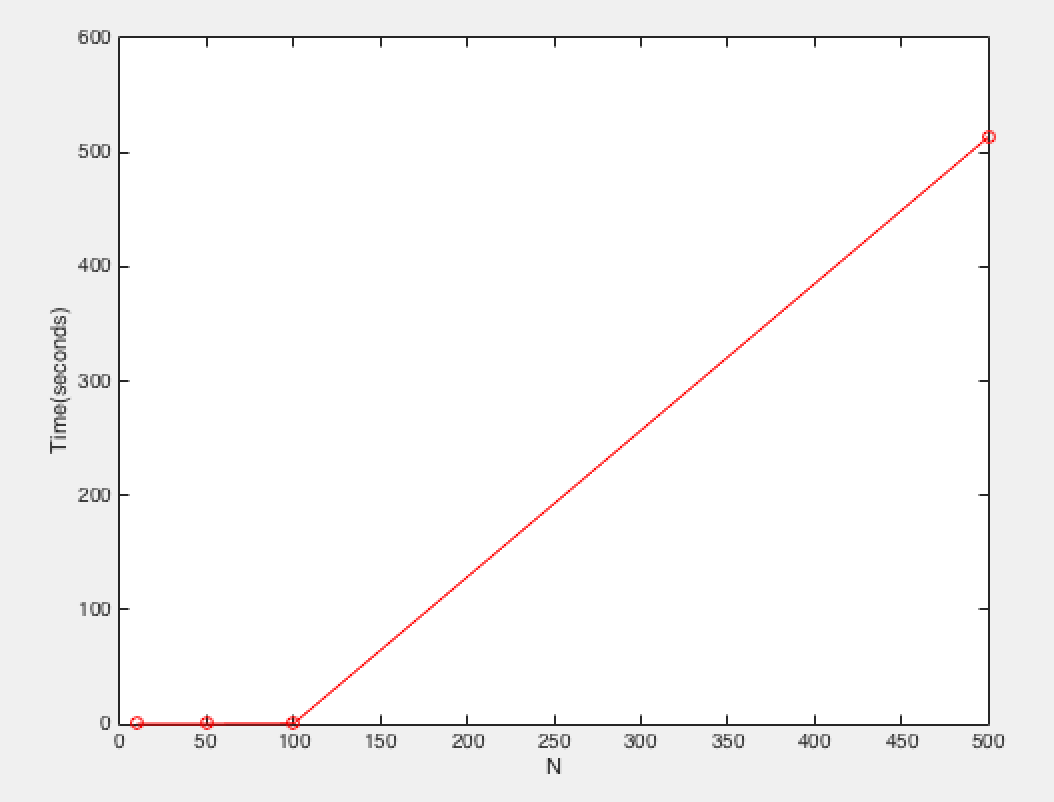
\includegraphics[width=0.7\textwidth]{method1} 
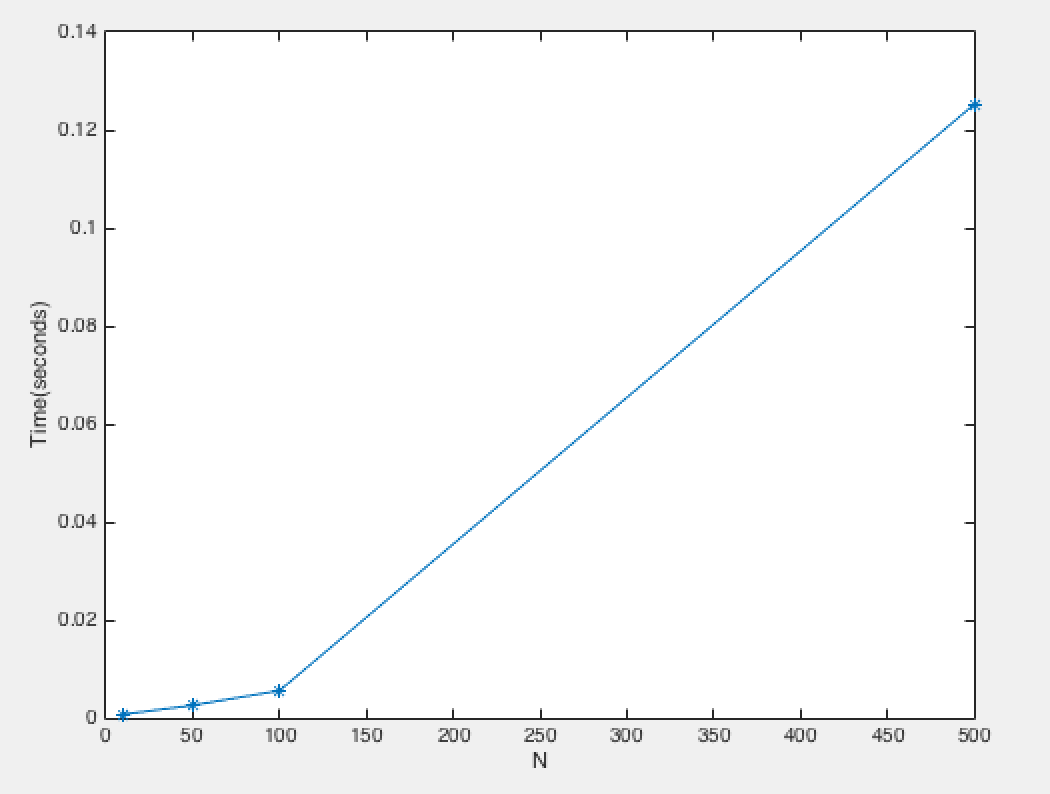
\includegraphics[width=0.7\textwidth]{method2} 



\item


\item 

Code: \\
\begin{lstlisting} 
function U= jacobian(A, b)
[N,t] = size(b); 
U = zeros(N,1) ; 
size(A) 
size(b) 
true = A\b; 
diff = 100; 
iter = 0 ; 
while diff > 1.0e-4 
    temp = U; 
    for i=1:N
        sum = 0; 
        for j=1:N
            if i~=j
                sum = sum + A(i,j)*temp(j); 
            end
        end
        U(i) = 1/A(i,i)*(b(i)-sum); 
    end
    diff  =  norm(U- true) ; 
    iter = iter + 1 ; 
end 

end
\end{lstlisting} 

\begin{table}[!htbp]
\centering
\caption{Problem2.5}
\label{my-label}
\begin{tabular}{|l|l|}
\hline
N   & Iteration \\ \hline
10  & 182       \\ \hline
50  &   4567        \\ \hline
100 &           \\ \hline
500 &           \\ \hline
\end{tabular}
\end{table}

\item 
The results are shown in the following tables for different right side vectors. \\
\begin{table}[!htbp]
\centering
\caption{$f(x, y)=1$ }
\label{my-label}
\begin{tabular}{|l|l|}
\hline
N   & Iteration \\ \hline
10  &        \\ \hline
50  &           \\ \hline
100 &           \\ \hline
500 &           \\ \hline
\end{tabular}
\end{table}

\begin{table}[!htbp]
\centering
\caption{$f(x, y)=-1$ }
\label{my-label}
\begin{tabular}{|l|l|}
\hline
N   & Iteration \\ \hline
10  &        \\ \hline
50  &           \\ \hline
100 &           \\ \hline
500 &           \\ \hline
\end{tabular}
\end{table}

\begin{table}[!htbp]
\centering
\caption{$f(x, y)=-(x-0.5)^2-(y-0.5)^2$ }
\label{my-label}
\begin{tabular}{|l|l|}
\hline
N   & Iteration \\ \hline
10  &        \\ \hline
50  &           \\ \hline
100 &           \\ \hline
500 &           \\ \hline
\end{tabular}
\end{table}

\begin{table}[!htbp]
\centering
\caption{$f(x, y)=sin(100x)cos(100y)$ }
\label{my-label}
\begin{tabular}{|l|l|}
\hline
N   & Iteration \\ \hline
10  &        \\ \hline
50  &           \\ \hline
100 &           \\ \hline
500 &           \\ \hline
\end{tabular}
\end{table}




\end{enumerate}




\end{document}
